\chapter{Rules of Schafkopf}
Schafkopf is a traditional four player trump card game that is played in the south of Germany.
The game is widely popular for being easy to learn but allowing for deep strategies.
Often it is played for small money stakes.
A game of Schafkopf normally consists of multiple rounds of four hands, where the intial dealer position rotates
clockwise around the table.
In Order to play a hand players will bid between themselves for a game contract, creating either two teams of two or
two teams of one and three, and then play 8 tricks with differing rules sets that depend on the winning bid.


\section{Cards}\label{sec:cards}
The Game of Schafkopf uses a 32 card bavarian deck, containing 4 suits with 8 ranks each.
Since the bavarian deck is comparable with a 52 french deck, where all ranks 2-6 are excluded, we also included the
corresponding English names for each suit and rank in the following tables.
The following tables is ordered descendingly by strength.
\begin{table}[]
    \begin{tabular}{lll}
        Suit     & Short Hand & Corresponding French Suit \\
        Eichel   & E          & Clubs                     \\
        Gras     & G          & Spades                    \\
        Herz     & H          & Hearts                    \\
        Schellen & S          & Diamonds
    \end{tabular}\label{tab:table2}
\end{table}
Regardless of the contract each rank has a corresponding point value ranging from 11 to 0 points in discrete steps.
The total value of all 32 cards is therefore 120.
\begin{table}[]
    \begin{tabular}{llll}
        Rank  & Point Value & Short Hand & Corresponding French Rank \\
        Ass   & 11          & A          & Ace                       \\
        Zehn  & 10          & T          & Ten                       \\
        König & 4           & K          & King                      \\
        Ober  & 3           & O          & Queen                     \\
        Unter & 2           & U          & Jack                      \\
        9     & 0           & 9          & Nine                      \\
        8     & 0           & 8          & Eight                     \\
        7     & 0           & 7          & Seven
    \end{tabular}\label{tab:table}
\end{table}
In order to refer to cards in the future we also included a short hand way of expressing suit and rank.
For example the Ten of Herz is TH and the Ober of Gras is OG.


\section{Goal and Rules}
\subsubsection{Goal}
The goal is to score points by taking tricks, of which there are eight.
If a team after all cards are played has 61 points (60 for the opposition) the game is won.
The rulesset for Schafkopf depends on the contract that is being played, there are however a certain rules that
always apply.
\subsubsection{Trumps}
Schafkopf has a set of cards that are considered trump.
This set of cards is determined by the contract that is played.
Each set has an order of strenght that always follows the order of Ober > Unter > Color.
The suits themselves have also an order of Eichel > Gras > Herz > Schellen.
As an example the order of trumps for the most common contract Team, where all Ober, all Unter and all Herz are trump:
(OE,OG,OH,OS,UE,UG,UH,US,AH,TH,KH,9H,8H,7H)
\subsubsection{Trick}
There are two kinds of tricks, trump and suit.
The first card of each trick,it can either be of trump or a normal suit, determines which kind is present.
In both cases players behind must play a card of that suit/trump.
If they do not possess one of that kind they may play any other card, even trump if the first card played is a suit.
\newline
A suit trick can be won either by having the highest card suit on the table or by having the highest trump on the table.
Trump tricks can however only be won by playing the highest trump.
There is no obligation to win a trick if you can do so.
Other restrictions and obligations on which cards can be played will be introduced in the Team contract section,
but the above rules are sufficient in most cases.
\section{Game Phases}
At the beginning of each player is seated at the table, and a player is randomly chosen to deal.
The initial seating relative to one another should not be changed, since the dealer position rotates after each hand
clockwise, thus
skewing the fairness.
\newline
Every hand of Schafkopf can be broken down in four distinct phases:
\begin{enumerate}
    \item Setup Phase
    \item Bidding Phase
    \item Trick Phase
    \item Scoring Phase
\end{enumerate}
To avoid complexity we excluded the doubling stage (players can choose to double the final hand reward after they
receive the first half of their hand), and the Contra stage (opposition players may double the stakes after the first card is played)
\subsection{Setup Phase}
At the beginning of a hand the player in the dealer position shuffles the cards and deals each player a hand of eight
cards.
This player is called the Dealer, and the player to his immediate left has the Lead.
\subsection{Bidding Phase}
The player with the lead starts the bidding phase and can either announce Pass or Play, then the next player clockwise announces his bid.
This continues until all players announced their intentions.
If a any previous player anounced Play, players may only also announce Play if they intend to chose a Solo Mode.
If every player passes, the hand ends and the current dealer reshuffels the cards and returns to
the Setup Phase.
If only one player announced Play, he announces his chosen contract and the Trick Phase begins.
If more than one player announced Play, the players with the highest bid wins the bid.
The order goes TEAM < WENZ < SOLO
\subsection{Trick Phase}
The player with the Lead plays his first card and the play continues in clockwise order until everybody played one
card.
The winner of the of the current trick collects all cards and becomes the new Lead.
After all eight tricks have been played the game moves into the scoring phase.
\subsection{Scoring Phase}
Each team counts their combined points, and a winner is determined.
The team that won the bid requires 61 points, whilst the opposition team only requires 60 points.
The rewards can now be calculated using a prearranged structure.
The base value of a game depends on the contract
that is being played,where SOLO modes are rewarded more due to their higher risk.
\newline
There are also specials rewards a team can earn:
\begin{description}
    \item[Schneider] The bid winners can claims Schneider when the opposition has not scored 30 points and vice versa
    if the bid winners have not scored 31 points.
    \item[Schwarz] A winning team can claim Schwarz if the other team have not won a single trick. A trick with 0
    points still counts as trick win.
    \item[Laufende] Laufende is a row of the highest trumps held by a party without interruption.
    In the TEAM game and COLOR Solo, payment is made from three Laufende (at least OE,OG,OH) and in the WENZ,
    payment is made from two Laufende (at leas UE,UG). Laufende can range from 2 up to 14 depening which contract is
    played.
\end{description}
The formula to calculate the final hand reward is always:
\begin{equation*}
    Hand Reward = Base Reward + Schneider + Schwarz + Laufende
\end{equation*}
Losers pay the winner the Hand rewards paid out always sum up to zero.
In TEAM game the losers get the negative hand reward, and the winners receive the positive hand reward.
In SOLO the bid winner receives three time the reward and each player receives a single hand reward.
The structure used in this paper can be found in the following table.
The hand is now finished, and the dealer role rotates clockwise.
\begin{table}[]
\begin{tabular}{ll}
Name     & Base Reward \\
Specials & 10          \\
Team     & 20          \\
Solo     & 50    
\end{tabular}\label{tab:table3}
\end{table}
\section{Contracts}
Schafkopf has a lot of differing contracts,these often allow for more Solo contracts or avoid aborting the hand.
All contracts follow the same trick rules we defined ealier, and only differ in the way the players are divided in
teams,what cards are Trump and the order of card ranks.
For this implementation we considered only the three classic contracts:
\begin{itemize}
    \item Team Mode
    \item Wenz
    \item Color Solo
\end{itemize}
Team mode is a two vs two variant and most, whilst WENZ and COLOR SOLO both pit the bid winner against the other three.

\subsection{Team}
In the Team game there are 14 Trumps, four Ober, four Unter and all Herz.
\newline
The bid winner calls a color ace that she does not hold herself, but she must hold at least one card of that color
that is not trump.
The player that holds the ace, being called the partner, will be allied for with the bid winner, whilst the remaining
players form the opposition team.
\newline
\begin{figure}
    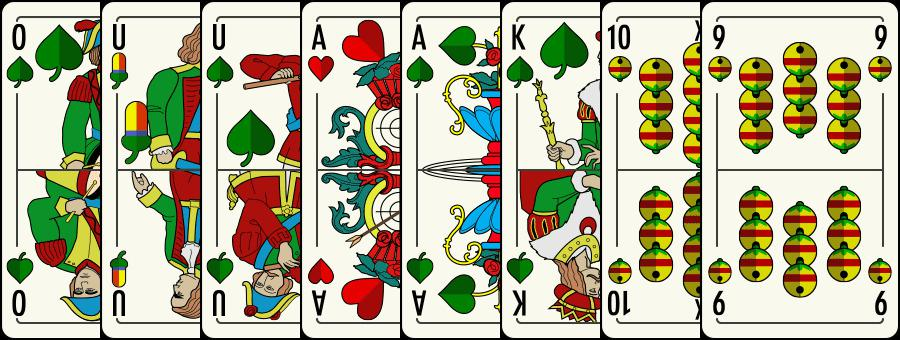
\includegraphics[scale=0.5]{partnerBiddingExample}\label{fig:figure}
\end{figure}
At the beginning of the hand only the partner knows the full team compositions, but in normal play this becomes
apparent fairly soon, can sometimes however last until the last trick.
If a trick starts with the searched color, the Partner has to play the ace.
This process is called Searching and reveals the team composition.
The partner may play the Ace at the beginning of a trick himself if he has the lead.
If no one searches the ace may only be played in the last trick.
If the partner has a four cards of the searched suit,including the ace, he may run away by playing a different card of
that suit, if and only if he has the lead.
Once runaway he may play the ace at any point.
This is due to the fact that if he holds 4 cards of the suit, the bid winner one, there is only one remaining cards
with the opposition.
This would guarantee a lost trick if the opposition searches and holds trump.

\subsection{Solos}
The Solos require a much stronger hand in general in order to win.

\subsubsection{Suit Solo}
The bid winner calls which color is trump.
As with the Team game there are 14 Trumps, four Ober, four Unter and six cards of the chosen color.
The team composition is obvious after the bid winner announces his game.

\subsubsection{Wenz Solo}
In the Wenz Solo the only trumps are the four Unter.
The Ober are now considered color and slot in after the King in terms of card ranking.


\section{Basic Strategy}
Schafkopf is a game with a lot of subtle and deep strategies that can take a many hands to master, yet most beginners
are given a set of base rules to follow.
Most of these rules are role dependent and will be outlined shortly below.

\subsection{Bidder plays Trump,oppositon plays color}
This rule refers to the decision when a player has the lead.
